\chapter{Результаты исследований}\label{ch:ch7}

Исследовано было 6 образцов грунтов на минеральный состав, 18 образцов 
на гранулометрический состав, 25 образцов на физические свойства и 
проведено 15 компрессионных испытаний.

\section{Минеральный состав}

Минеральный состав исследуемых грунтов был определен путем проведения 
рентгено-структурного 
анализа, который сделан работниками кафедры  инженерной и экологической геологии 
геологического факультета МГУ им.М.В.Ломоносова
инж. 1 кат. С.А. Гараниной, вед. инж. С.В. Закусиным, ст.н.с., к.г.-м.н. В.В. Крупской.
Рентгеновские дифракционные картины представлены в приложении \ref{app:difrac}.

По результатам анализа составлена таблица \ref{tab:mineral}, отражающая минеральный состав 
исследованных грунтов.

\begin{table}[h!]
  \small
    \centering
  \begin{threeparttable}
  \caption{Минеральный состав исследованных грунтов (вес. \%)}
  \label{tab:mineral}
    \begin{tabular}{|l|c|c|c|c|c|c|}
        \hline
                                  & GJ68B7 & GJ68D4 & GJ6881 & GJ6890 & GJ6898 & GJ6899 \\ \hline
    Хлорит                        & 1,9  & 3,9  & 2,3  & 2,9  & 2,4  & 1,4  \\ \hline
    Смектит*                      & 14,3 & 13,2 & 34,7 & 32,9 & 22,0 & 15,0 \\ \hline
    Иллит                         & 8,8  & 4,8  & 5,9  & 4,3  & 5,2  & 6,2  \\ \hline
    Палыгорскит**                 & 1,0  & 0,1  & 0,0  & 0,0  & 0,0  & 0,0  \\ \hline
    Каолинит                      & 3,6  & 1,9  & 2,8  & 1,8  & 1,1  & 2,7  \\ \hline
    Кварц                         & 44,1 & 53,0 & 35,0 & 40,1 & 47,4 & 48,7 \\ \hline
    КПШ (микроклин, ортоклаз)     & 8,7  & 9,0  & 8,7  & 5,6  & 11,9 & 14,4 \\ \hline
    Плагиоклазы (альбит, андезит) & 3,3  & 7,3  & 6,7  & 11,5 & 7,9  & 8,4  \\ \hline
    Кальцит                       & 6,2  & 2,1  & 0,8  & 0,3  & 0,0  & 0,4  \\ \hline
    Доломит                       & 7,7  & 2,9  & 1,1  & 0,2  & 0,0  & 0,0  \\ \hline
    Сидерит                       & 0,0  & 0,0  & 0,0  & 0,0  & 0,3  & 0,4  \\ \hline
    Рутил                         & 0,0  & 0,0  & 0,4  & 0,4  & 0,0  & 0,9  \\ \hline
    Пирит                         & 0,4  & 0,3  & 0,3  & 0,0  & 0,4  & 0,4  \\ \hline
    Амфиболиты (роговая обманка)  & 0,0  & 1,5  & 1,3  & 0,0  & 1,4  & 1,1  \\ \hline
    \end{tabular}
    \raggedright 
    * Вероятно присутствие смешанослойного минерала иллит-смектит с~преобладанием смектитовых 
    (набухающих) пакетов. 
    Для точной диагностики требуется выделение глинистой фракции.
    \\
    ** Присутствие палыгорскита требует уточнения путем анализа глинистой фракции
    \\
    ***Образцы GJ68B7 и GJ68D4 относятся к ИГЭ-9 (суглинки полутвердые), GJ6881 и GJ6890 --- ИГЭ-8а (глины полутвердые), 
    GJ6898 и GJ6899 --- ИГЭ-7 (суглинки тугопластичные).
    \end{threeparttable}
    \end{table}

%Образцы GJ68B7 и GJ68D4 относятся к 9 инженерно-геологическому 
%элементу (суглинки полутвердые), GJ6881 и GJ6890 --- 8-ИГЭ (глины полутвердые), 
%GJ6898 и GJ6899 --- 7-ИГЭ (суглинки тугопластичные).

По данным из таблицы \ref{tab:mineral} видно, что в грунтах преобладают такие 
минералы, как кварц (среднее содержание 44,7\%) и смектит (22\%). Напротив, минералов 
палыгорскит (0,18\%), сидерит (0,12\%), рутил (0,28\%) и пирит (0,3\%) 
практически нет ни в одном образце. 

%Также в лаборатории были построены ренгеновские дифракционные 
%картины, представленные в Приложении \ref{app:difrac}. 

\section{Гранулометрический состав}

Гранулометрический состав грунтов был определен ареометрическим 
методом только для песчаной и глинистой фракций, не учитывая 
крупнообломочную фракцию. 

По результатам анализа на гранулометрический состав 
построены интегральные (кумулятивные) кривые (рис. \ref{fig:curves}) и 
треугольная диаграмма гранулометрического состава Ферре (рис. \ref{Fig:Ferre}).


{
\small
\pgfplotsset{
%samples=15,
width=0.45\linewidth,
xlabel={Диаметр частиц $d$, мм},
ylabel={Содержание частиц, \%},
%extra y ticks={45},
legend pos=north west,
ymin = 0,
ymax = 100,
}

\begin{figure}
	{\centering
	\small
	\subbottom[ИГЭ-6 (суглинки тугопластичные)]{\begin{tikzpicture}
    \begin{semilogxaxis}[]
    
    % ИГЭ-6
    \addplot[smooth, no marks, red!70!orange!80!black] table [x=Size, y=GJ6805, col sep=semicolon] {data/hydrometer-cumulative.csv};
    \addplot[smooth, no marks, red!70!orange!80!black] table [x=Size, y=GJ6807, col sep=semicolon] {data/hydrometer-cumulative.csv};
    \addplot[smooth, no marks, red!70!orange!80!black] table [x=Size, y=GJ6838, col sep=semicolon] {data/hydrometer-cumulative.csv};
    \addplot[smooth, no marks, red!70!orange!80!black] table [x=Size, y=GJ6835, col sep=semicolon] {data/hydrometer-cumulative.csv};
    
    \end{semilogxaxis}
\end{tikzpicture}}
	\hfill
	\subbottom[ИГЭ-7 (суглинки тугопластичные)]{\begin{tikzpicture}
    \begin{semilogxaxis}[]
    
    % ИГЭ-7
    \addplot[smooth, no marks, lime!40!black] table [x=Size, y=GJ6898, col sep=semicolon] {data/hydrometer-cumulative.csv};
    \addplot[smooth, no marks, lime!40!black] table [x=Size, y=GJ6874, col sep=semicolon] {data/hydrometer-cumulative.csv};
    
    \end{semilogxaxis}
\end{tikzpicture}
}
	}
	\\
	{\centering
	\small
	\subbottom[ИГЭ-8а (глины полутвердые)]{\begin{tikzpicture}
    \begin{semilogxaxis}[]
    
    % ИГЭ-8
    \addplot[smooth, no marks, green!10!lime!30!black] table [x=Size, y=GJ6822, col sep=semicolon] {data/hydrometer-cumulative.csv};
    \addplot[smooth, no marks, green!10!lime!30!black] table [x=Size, y=GJ6884, col sep=semicolon] {data/hydrometer-cumulative.csv};
    \addplot[smooth, no marks, green!10!lime!30!black] table [x=Size, y=GJ6846, col sep=semicolon] {data/hydrometer-cumulative.csv};
    \addplot[smooth, no marks, green!10!lime!30!black] table [x=Size, y=GJ6890, col sep=semicolon] {data/hydrometer-cumulative.csv};
    \addplot[smooth, no marks, green!10!lime!30!black] table [x=Size, y=GJ6888, col sep=semicolon] {data/hydrometer-cumulative.csv};
    
    
    \end{semilogxaxis}
\end{tikzpicture}}
	\hfill
	\subbottom[ИГЭ-9 (суглинки полутвердые)]{\begin{tikzpicture}
    \begin{semilogxaxis}[]
    
    % ИГЭ-9
    \addplot[smooth, no marks, red!80!orange!50!black] table [x=Size, y=GJ6865, col sep=semicolon] {data/hydrometer-cumulative.csv};
    \addplot[smooth, no marks, red!80!orange!50!black] table [x=Size, y=GJ68A3, col sep=semicolon] {data/hydrometer-cumulative.csv};
    \addplot[smooth, no marks, red!80!orange!50!black] table [x=Size, y=GJ68B7, col sep=semicolon] {data/hydrometer-cumulative.csv};
    \addplot[smooth, no marks, red!80!orange!50!black] table [x=Size, y=GJ68A0, col sep=semicolon] {data/hydrometer-cumulative.csv};
    
    \end{semilogxaxis}
\end{tikzpicture}}
	}

	\caption{Кумулятивные кривые гранулометрического состава исследованных грунтов}
	\label{fig:curves}
	%\raggedright 
	%* ИГЭ-6 --- суглинки тугопластичные, ИГЭ-7 --- суглинки тугопластичные,
	%ИГЭ-8а --- глины полутвердые, ИГЭ-9 --- суглинки полутвердые.
\end{figure}
}


\begin{figure}[h!]
  {\centering
  \small
  %\pgfplotstableset{format=file}
\pgfplotsset{width=0.6\linewidth}

\begin{tikzpicture}
    \begin{ternaryaxis}[
        legend cell align={left},
        %title=Spinel,
        ternary limits relative=false,
        %width=10cm,
        %height=10cm,
        xmax=100,
        ymax=100,
        zmax=100,
        minor tick num=1,
        grid=both,
        xlabel={Глина, \%},
        xlabel style={
            at={(axis cs:100,0,0)},
            anchor=south,
            yshift=16pt,
            align=center
        },
        ylabel={Песок, \%},
        ylabel style={
            at={(axis cs:0,100,0)},
            anchor=10,
            xshift=-11pt,
            yshift=-16pt,
            align=center
        },
        zlabel={Пыль, \%},
        zlabel style={
            at={(axis cs:0,0,100)},
            anchor=north west,
            xshift=16pt,
            yshift=-11pt,
            align=center
        },
    ]

        \addplot3 [only marks, mark=*, red!70!orange!80!black] 
        table [x=Clay, y=Sand, z=Silt, col sep=semicolon, row sep=newline] {data/gran-activity-6.csv};
        \addlegendentry{ИГЭ-6}

        \addplot3 [only marks, mark=*, lime!50!yellow!40!black]
        table [x=Clay, y=Sand, z=Silt, col sep=semicolon, row sep=newline] {data/gran-activity-7.csv};
        \addlegendentry{ИГЭ-7}

        \addplot3 [only marks, mark=*, green!50!lime!30!black] 
        table [x=Clay, y=Sand, z=Silt, col sep=semicolon, row sep=newline] {data/gran-activity-8.csv};
        \addlegendentry{ИГЭ-8а}

        \addplot3+[only marks, mark=*, red!80!orange!50!black] 
        table [x=Clay, y=Sand, z=Silt, col sep=semicolon, row sep=newline] {data/gran-activity-9.csv};
        \addlegendentry{ИГЭ-9}

    \end{ternaryaxis}
\end{tikzpicture}
  \caption{Треугольная диаграмма Ферре для выражения гранулометрического состава исследованных грунтов}
  \label{Fig:Ferre}
  \raggedright 
  * ИГЭ-6 --- суглинки тугопластичные, ИГЭ-7 --- суглинки тугопластичные,
  ИГЭ-8а --- глины полутвердые, ИГЭ-9 --- суглинки полутвердые.}
\end{figure}

Анализируя полученные результаты, можно полагать: 
в среднем для ИГЭ-6 (суглинки тугопластичные) характерен следующий состав: $\thicksim$63\% песчаных,
$\thicksim$26\% пылеватых и $\thicksim$11\% глинистых частиц; 
для ИГЭ-7 (суглинки тугопластичные) --- $\thicksim$20\% песчаных, $\thicksim$58\% пылеватых и $\thicksim$22\% глинистых частиц; 
для ИГЭ-8а (глины полутвердые) --- $\thicksim$35\% песчаных, $\thicksim$45\% пылеватых и $\thicksim$20\% глинистых частиц; 
для ИГЭ-9 (суглинки полутвердые) --- $\thicksim$61\% песчаных, $\thicksim$23\% пылеватых и $\thicksim$16\% глинистых частиц.
По классификации В.В.Охотина "Классификация дисперсных грунтов по гранулометрическому составу" 
можно назвать грунты каждого инженерно-геологического элемента 
следующим образом: ИГЭ-6 (суглинки тугопластичные) --- суглинок легкий, ИГЭ-7
 (суглинки тугопластичные) --- суглинок тяжелый
пылеватый, ИГЭ-8а (глины полутвердые) --- суглинок тяжелый пылеватый, 
ИГЭ-9 (суглинки полутвердые) --- суглинок средний 
(Лабораторный практикум по грунтоведению: Учебное пособие, 2019).

Сопостовляя результаты рентгено-структурного анализа и гранулометрического, 
можно прийти к выводу, что содержание песка в образцах соотносится с 
содержанием кварца, пылеватых частиц "--- плагиоклазов и калиевых
полевых шпатов, а содержание глинистых частиц примерно сопоставляется с 
содержанием иллита, смектита, каолинита, хлорита и других глинистых минералов.

\section{Физические свойства}

Результаты опытов по определению физических свойств представлены в 
Приложении \ref{app:phisics}. 

В итоге по инженерно-геологическим элементам получились следующие 
средние значения плотности грунта: 
ИГЭ-6 (суглинки тугопластичные) --- 2,17 г/\si{\centi\meter^3}, 
ИГЭ-7 (суглинки тугопластичные) --- 2,00 г/\si{\centi\meter^3}, 
ИГЭ-8а (глины полутвердые) --- 2,05 г/\si{\centi\meter^3}, 
ИГЭ-9 (суглинки полутвердые) --- 2,15 г/\si{\centi\meter^3}; 
значения плотности твердых частиц: 
ИГЭ-6 (суглинки тугопластичные) --- 2,70 г/\si{\centi\meter^3}, 
ИГЭ-7 (суглинки тугопластичные) --- 2,72 г/\si{\centi\meter^3}, 
ИГЭ-8а (глины полутвердые) --- 2,72 г/\si{\centi\meter^3}, 
ИГЭ-9 (суглинки полутвердые) --- 2,71 г/\si{\centi\meter^3}. 
Средние значения естественной влажности для каждого элемента:
ИГЭ-6 (суглинки тугопластичные) --- 16\% соответственно, 
ИГЭ-7 (суглинки тугопластичные) --- 25\%, 
ИГЭ-8а (глины полутвердые) --- 22\%, 
ИГЭ-9 (суглинки полутвердые) --- 17\%.
Средние значения верхнего и нижнего пределов пластичности 
получились такие: 
ИГЭ-6 (суглинки тугопластичные) --- 22 и 12 \% соответственно, 
ИГЭ-7 (суглинки тугопластичные) --- 33 и 20 \%, 
ИГЭ-8а (глины полутвердые) --- 43 и 19 \%, 
ИГЭ-9 (суглинки полутвердые) --- 33 и 15 \%.
Средние значения числа пластичности и показателя текучести 
для каждого инженерно-геологического элемента получились такие:
ИГЭ-6 (суглинки тугопластичные) --- 0,10 и 0,35 д.~е. соответственно, 
ИГЭ-7 (суглинки тугопластичные) --- 0,13 и 0,37 д.~е., 
ИГЭ-8а (глины полутвердые) --- 0,24 и 0,13 д.~е., 
ИГЭ-9 (суглинки полутвердые) --- 0,18 и 0,12 д.~е.
В соответствии с классификацией ГОСТ 25100-2011 
по числу пластичности и показателю текучести 
грунты получаются следующие:
ИГЭ-6 --- суглинок тугопластичный;
ИГЭ-7 --- суглинок тугопластичный;
ИГЭ-8а --- глина полутвердая;
ИГЭ-9 --- глина полутвердые.
Получились различия в определении грунта по сравнению 
с производственными данными только для 
ИГЭ-9. Это может объясняться тем, что на производстве 
было исследовано много большее количесество образцов, 
поэтому средние показатели указали на другой 
тип грунта.

Средние значения коэффициента пористости и 
степени водонасыщения по инженерно-геологическим 
элементам получились следующие:
ИГЭ-6 (суглинки тугопластичные) --- 0,44 и 0,95 д.~е. соответственно, 
ИГЭ-7 (суглинки тугопластичные) --- 0,69 и 0,96 д.~е., 
ИГЭ-8а (глины полутвердые) --- 0,63 и 0,97 д.~е., 
ИГЭ-9 (суглинки полутвердые) --- 0,48 и 0,94 д.~е.

На рисунке \ref{fig:plgl} изображен график зависимости плотности 
грунта от глубины залегания. Видно, что в целом прослеживается 
закономерность --- с увеличением глубины увеличивыется и 
плотность грунта.

\begin{figure}[ht]
  \centerfloat{
    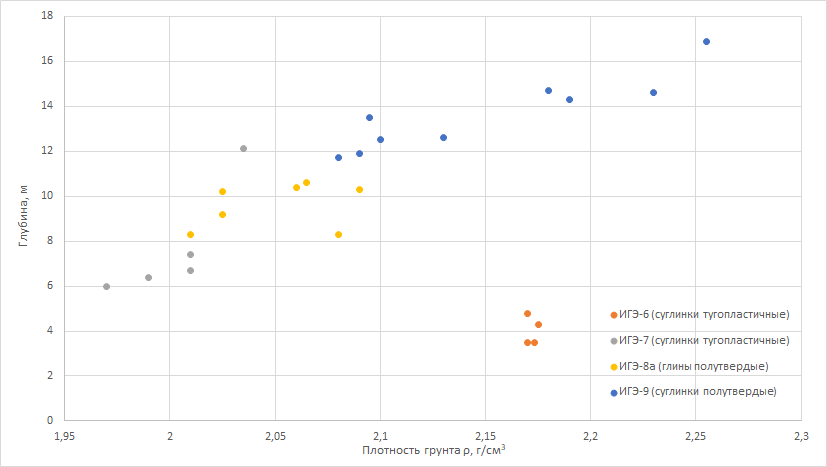
\includegraphics[scale=1]{plgl(4).png}
  }
  \caption{График зависимости плотности грунта от глубины залегания}\label{fig:plgl}
\end{figure}

На рисунке \ref{fig:vlgl} показана зависимость 
естественной влажности грунта $W$, \% от его глубины залегания.
Здесь также видна закономерность уменьшения естественной 
влажности от глубины залегания.

\begin{figure}[ht]
  \centerfloat{
    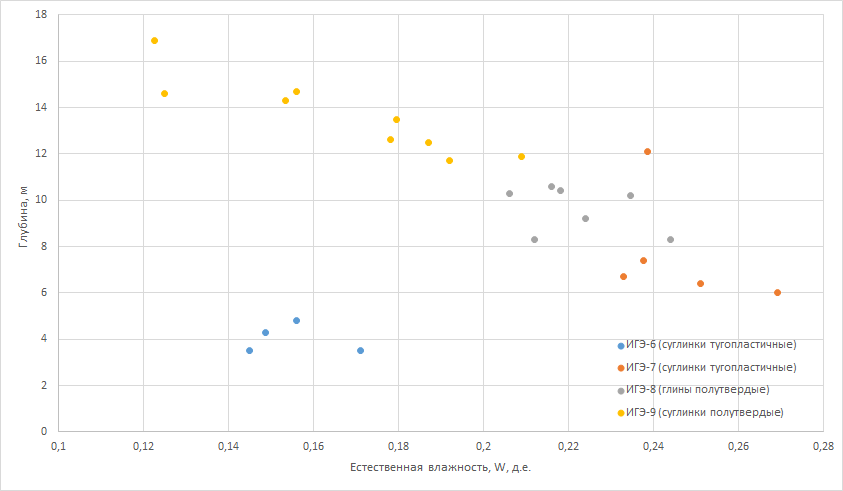
\includegraphics[scale=1]{vlgl.png}
  }
  \caption{График зависимости естественной влажности грунта от глубины залегания}\label{fig:vlgl}
\end{figure}

\section{Физико-механические свойства}

\subsection{Компрессионное сжатие}

Результаты компрессионного сжатия, 
компрессионные кривые, представлены в 
приложении \ref{app:oedometer}.

\subsection{Параметры переуплотнения}

Проведя компрессионное сжатие для образцов грунта, были построены 
графики в координатах вертикального напряжения $\sigma$ и коэффициента пористости $e$ 
в полулогарифмическом масштабе и вертикального напряжения $\sigma$ 
и энергии $W$ для определения напряжения предуплотнения 
методами Казагранде и Беккера соответственно. Были проведены 
графические построения для каждого образца по обоим 
методам, построения приведены в Приложении \ref{app:method}.

После построения графиков и их обработки, были определены 
напряжения предуплотнения $\sigma_c$, кПа двумя методами ---
Казагранде и Беккера. 
Напряжения предуплотнения, в свою очередь, использовались для расчета 
других характеристик переуплотнения: напряжение 
переуплотнения $POP$ и коэффициент переуплотнения $OCR$.
Для расчетов также понадобился еще один показатель "--- 
"бытовое"\ напряжение.

Характеристики переуплотнения, полученные по методу Казагранде и Беккера,
представленны в таблице \ref{tab:komp1} и таблице \ref{tab:komp2} соответственно.

\begin{table}[]
  \small
  \centering
  \begin{threeparttable}
    \caption{Параметры переуплотнения. Метод Беккера}\label{tab:komp2}
  \begin{tabular}{|p{1.7cm}|p{1.7cm}|p{5cm}|p{1.4cm}|p{1.4cm}|p{1.4cm}|p{1.4cm}|}
  \hline
  Образец & Глубина отбора & Наименование грунта & $\sigma_0$, \si{\kilo\Pa} & $\sigma_c$, \si{\kilo\Pa} & $POP$, \si{\kilo\Pa}   & $OCR$ \\ \hline
  GJ6805 & 3,5            & суглинок легкий\linebreak тугопластичный  & 70,0  & 195,0 & 125,0 & 2,8 \\ \hline
GJ6807 & 4,8            & суглинок легкий\linebreak тугопластичный  & 96,0  & 250,0 & 154,0 & 2,6 \\ \hline
GJ6838 & 4,3            & суглинок легкий\linebreak тугопластичный  & 86,0  & 240,0 & 154,0 & 2,8 \\ \hline
GJ6809 & 6              & суглинок\linebreak   мягкопластичный        & 120,0 & 310,0 & 190,0 & 2,6 \\ \hline
GJ6810 & 6,4            & суглинок полутвердый              & 128,0 & 410,0 & 282,0 & 3,2 \\ \hline
GJ6821 & 6,7            & суглинок   тугопластичный         & 134,0 & 398,0 & 264,0 & 3,0 \\ \hline
GJ6898 & 12,1           & суглинок тяжелый\linebreak тугопластичный & 242,0 & 330,0 & 88,0  & 1,4 \\ \hline
GJ6822 & 8,3            & глина полутвердая                 & 166,0 & 410,0 & 244,0 & 2,5 \\ \hline
GJ6884 & 9,2            & глина легкая   полутвердая        & 184,0 & 430,0 & 246,0 & 2,3 \\ \hline
GJ6846 & 8,3            & глина тяжелая\linebreak полутвердая       & 166,0 & 580,0 & 414,0 & 3,5 \\ \hline
GJ6855 & 11,7           & глина легкая   полутвердая        & 234,0 & 390,0 & 156,0 & 1,7 \\ \hline
GJ6859 & 12,5           & глина полутвердая                 & 250,0 & 440,0 & 190,0 & 1,8 \\ \hline
GJ6865 & 14,7           & глина легкая   полутвердая        & 294,0 & 830,0 & 536,0 & 2,8 \\ \hline
GJ68A3 & 13,5           & глина легкая   полутвердая        & 270,0 & 710,0 & 440,0 & 2,6 \\ \hline
GJ68B7 & 16,9           & суглинок тяжелый\linebreak   твердый        & 338,0 & 1060  & 722,0 & 3,1 \\ \hline
  \end{tabular}
\end{threeparttable}
  \end{table}

  \begin{table}[]
    \small
    \centering
    \begin{threeparttable}
      \caption{Параметры переуплотнения. Метод Казагранде}\label{tab:komp1}
    \begin{tabular}{|p{1.7cm}|p{1.7cm}|p{5cm}|p{1.4cm}|p{1.4cm}|p{1.4cm}|p{1.4cm}|}
    \hline
    Образец  & Глубина отбора & Наименование грунта & $\sigma_0$, \si{\kilo\Pa} & $\sigma_c$, \si{\kilo\Pa} & $POP$, \si{\kilo\Pa}   & $OCR$ \\ \hline
    GJ6805 & 3,5            & суглинок легкий   тугопластичный  & 70,0  & 240,0  & 170,0 & 3,4 \\ \hline
GJ6807 & 4,8            & суглинок легкий\linebreak   тугопластичный  & 96,0  & 240,0  & 144,0 & 2,5 \\ \hline
GJ6838 & 4,3            & суглинок легкий\linebreak   тугопластичный  & 86,0  & 310,0  & 224,0 & 3,6 \\ \hline
GJ6809 & 6              & суглинок\linebreak   мягкопластичный        & 120,0 & 370,0  & 250,0 & 3,1 \\ \hline
GJ6810 & 6,4            & суглинок полутвердый              & 128,0 & 470,0  & 342,0 & 3,7 \\ \hline
GJ6821 & 6,7            & суглинок   тугопластичный         & 134,0 & 440,0  & 306,0 & 3,3 \\ \hline
GJ6898 & 12,1           & суглинок тяжелый\linebreak   тугопластичный & 242,0 & 460,0  & 218,0 & 1,9 \\ \hline
GJ6822 & 8,3            & глина полутвердая                 & 166,0 & 500,0  & 334,0 & 3,0 \\ \hline
GJ6884 & 9,2            & глина легкая   полутвердая        & 184,0 & 450,0  & 266,0 & 2,4 \\ \hline
GJ6846 & 8,3            & глина тяжелая\linebreak полутвердая       & 166,0 & 650,0  & 484,0 & 3,9 \\ \hline
GJ6855 & 11,7           & глина легкая   полутвердая        & 234,0 & 430,0  & 196,0 & 1,8 \\ \hline
GJ6859 & 12,5           & глина полутвердая                 & 250,0 & 540,0  & 290,0 & 2,2 \\ \hline
GJ6865 & 14,7           & глина легкая   полутвердая        & 294,0 & 1170,0 & 876,0 & 4,0 \\ \hline
GJ68A3 & 13,5           & глина легкая   полутвердая        & 270,0 & 840,0  & 570,0 & 3,1 \\ \hline
GJ68B7 & 16,9           & суглинок тяжелый\linebreak   твердый         & 338,0 & 1215,0 & 877,0 & 3,6 \\ \hline
    \end{tabular}
  \end{threeparttable}
    \end{table}

Сопоставляя полученные данные разными методами, 
видно, что по методу Казагранде напряжения предуплотнения, 
следовательно, и рассчитанные параметры получились 
меньше, чем по методу Беккера для одних и тех же образцов.
Это можно объяснить тем, что каждое графическое построение 
выполняется индивидуально и результат сильно зависит от 
того, как автор изобразит вспомогательные элементы 
на графике такие, как касательные к прямолинейным участкам 
кривых и точку на максимальной кривизне графика.

Анализируя зависимости параметров переплотнения, 
полученные методом Казагранде, от глубины залегания 
(рис. \ref{fig:1gl}, \ref{fig:2gl}, \ref{fig:3gl}), 
видно, что небольшая зависимость прослеживается только  
на графиках зависимости $\sigma_c$ и $POP$ от глубины, на 
них параметры переуплотнения $\sigma_c$ и $POP$ увеличиваются 
с увеличением глубины. 

Точно такая же ситуация с характеристиками 
переуплотнения, полученными по методу Беккера (рис. \ref{fig:11gl}, \ref{fig:22gl}, \ref{fig:33gl}).

\begin{figure}[ht]
  \centerfloat{
    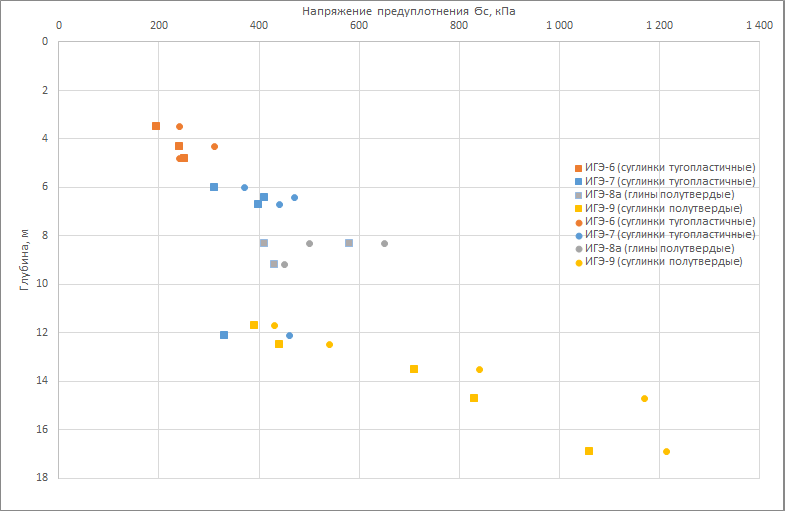
\includegraphics[scale=1]{1gl.png}
  }
  \caption{График зависимости напряжения предуплотнения $\sigma_c$ от глубины залегания (метод Казагранде)}\label{fig:1gl}
\end{figure}

\begin{figure}[h!]
  \centerfloat{
    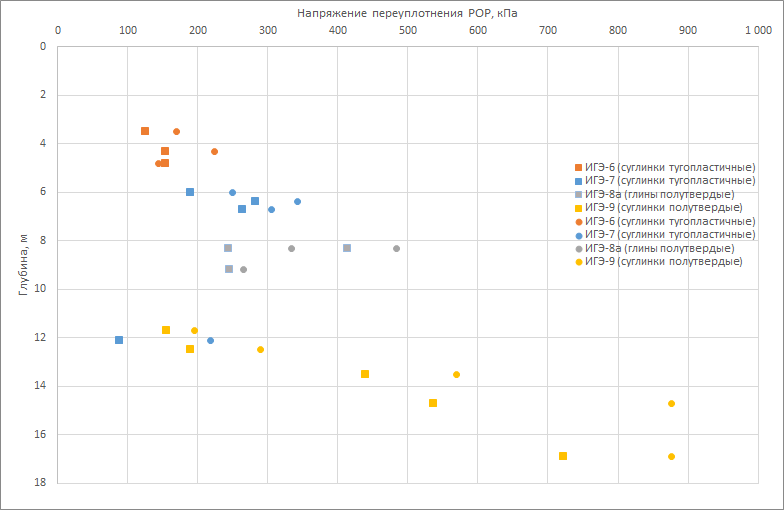
\includegraphics[scale=1]{2gl.png}
  }
  \caption{График зависимости напряжения переуплотнения $POP$ от глубины залегания (метод Казагранде)}\label{fig:2gl}
\end{figure}

\begin{figure}[h!]
  \centerfloat{
    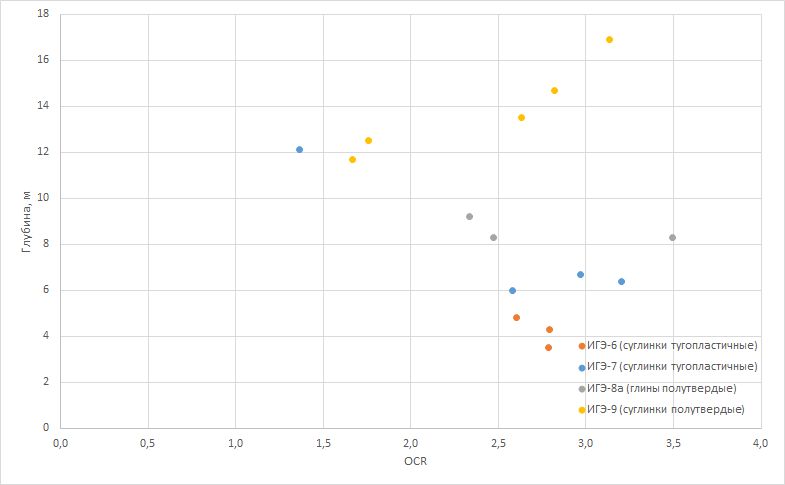
\includegraphics[scale=1]{3gl.png}
  }
  \caption{График зависимости коэффициента переуплотнения $OCR$ от глубины залегания (метод Казагранде)}\label{fig:3gl}
\end{figure}

\begin{figure}[h!]
  \centerfloat{
    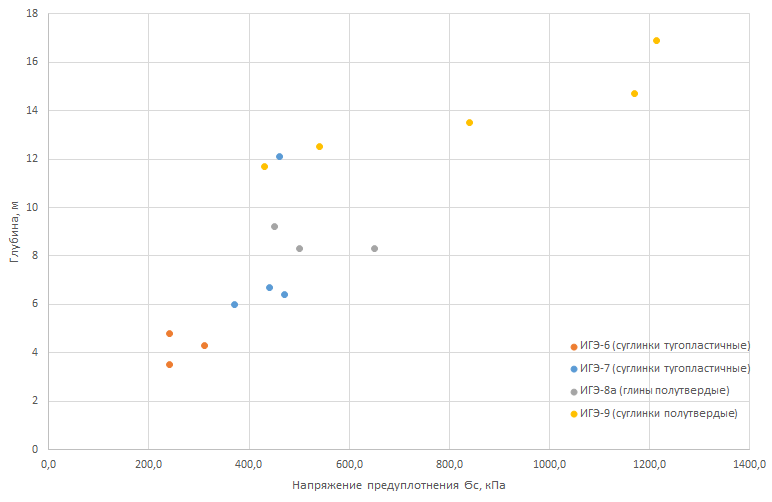
\includegraphics[scale=1]{11gl.png}
  }
  \caption{График зависимости напряжения предуплотнения $\sigma_c$ от глубины залегания (метод Беккера)}\label{fig:11gl}
\end{figure}

\begin{figure}[h!]
  \centerfloat{
    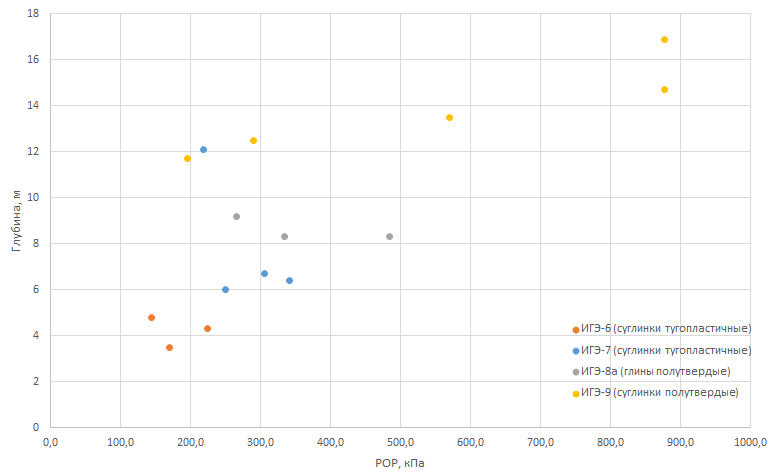
\includegraphics[scale=1]{22gl.png}
  }
  \caption{График зависимости напряжения переуплотнения $POP$ от глубины залегания (метод Беккера)}\label{fig:22gl}
\end{figure}

\begin{figure}[h!]
  \centerfloat{
    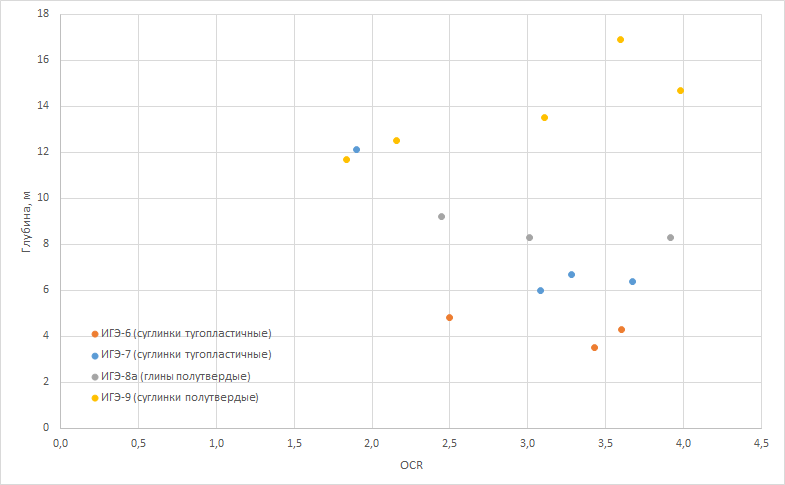
\includegraphics[scale=1]{33gl.png}
  }
  \caption{График зависимости коэффициента переуплотнения $OCR$ от глубины залегания (метод Беккера)}\label{fig:33gl}
\end{figure}

Так как значение напряжения переуплотнения $POP$
различно от напряжения предуплотнения $\sigma_c$ 
всегда на постоянную величину, в дальнейшем 
анализ будет только напряжения предуплотнения $\sigma_c$.

Напряжение предуплотнения $\sigma_c$ слабо 
зависит от естественной влажности грунта $W$ (рис. \ref{fig:1vl}, \ref{fig:3vl}), 
коэффициент переуплотнения совсем не зависит от 
влажности (рис. \ref{fig:11vl}, \ref{fig:33vl}).

\begin{figure}[h!]
  \centerfloat{
    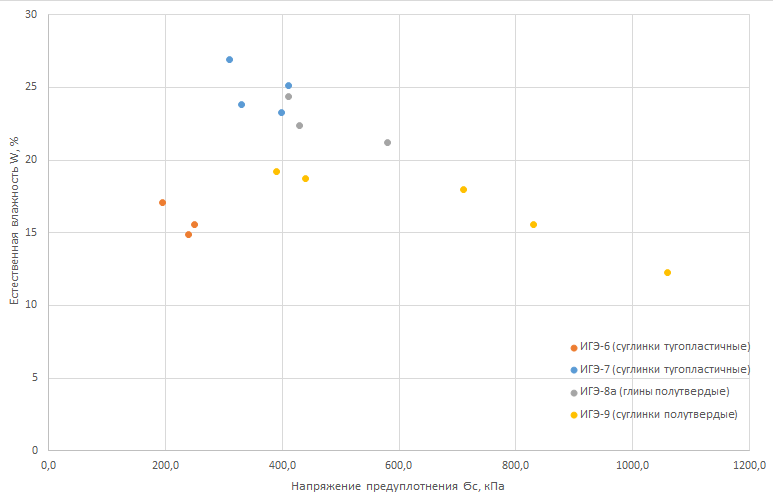
\includegraphics[scale=1]{1vl.png}
  }
  \caption{График зависимости напряжения предуплотнения $\sigma_c$ от естественной 
  влажности $W$ (метод Казагранде)}\label{fig:1vl}
\end{figure}

\begin{figure}[h!]
  \centerfloat{
    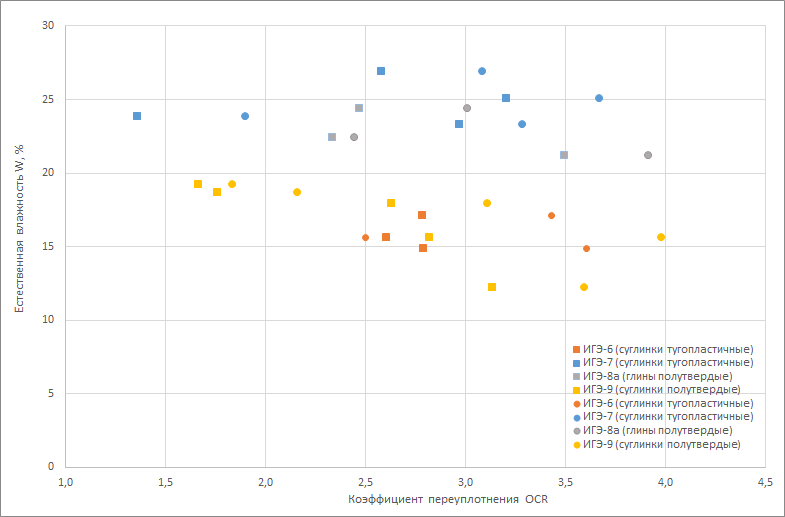
\includegraphics[scale=1]{3vl.png}
  }
  \caption{График зависимости коэффициента переуплотнения $OCR$ от 
  естественной 
  влажности $W$ (метод Казагранде)}\label{fig:3vl}
\end{figure}

\begin{figure}[h!]
  \centerfloat{
    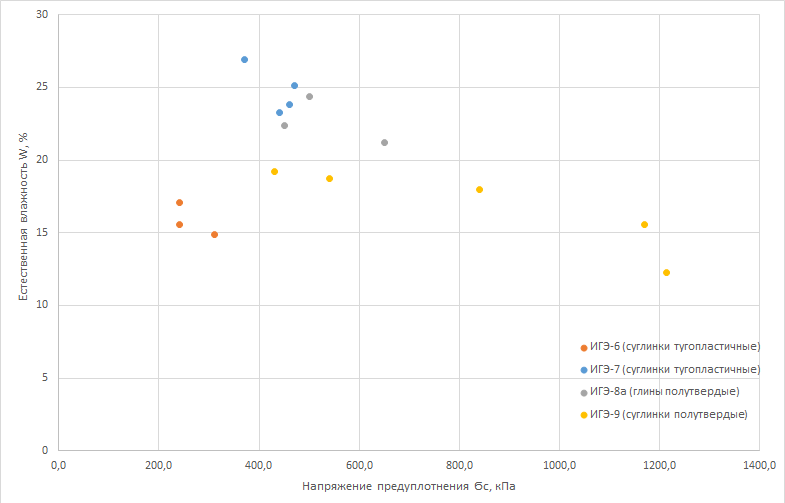
\includegraphics[scale=1]{11vl.png}
  }
  \caption{График зависимости напряжения предуплотнения $\sigma_c$ от 
  естественной 
  влажности $W$ (метод Беккера)}\label{fig:11vl}
\end{figure}

\begin{figure}[h!]
  \centerfloat{
    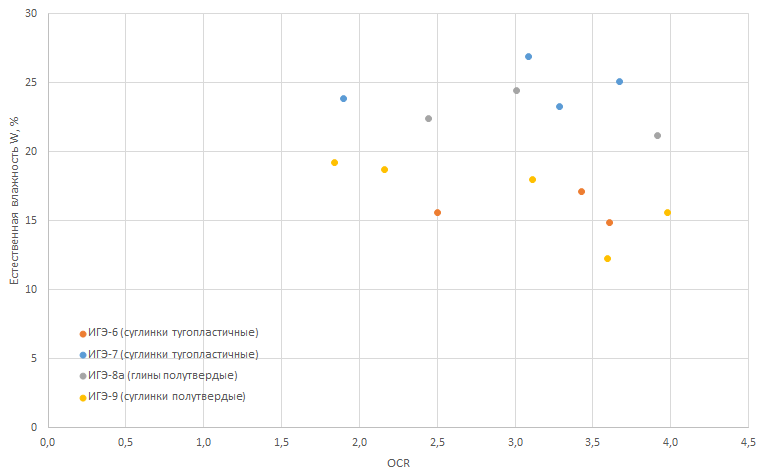
\includegraphics[scale=1]{33vl.png}
  }
  \caption{График зависимости коэффициента переуплотнения $OCR$ от 
  естественной 
  влажности $W$ (метод Беккера)}\label{fig:33vl}
\end{figure}

Зависимости между напряжением предуплотнения $\sigma_c$ 
и коэффициентом пористости $e$ нет, также 
ее нет и между коэффициентами переуплотнения $OCR$ и пористости $e$ (рис. \ref{fig:1por}, \ref{fig:3por}, \ref{fig:11por}, \ref{fig:33por}).

\begin{figure}[h!]
  \centerfloat{
    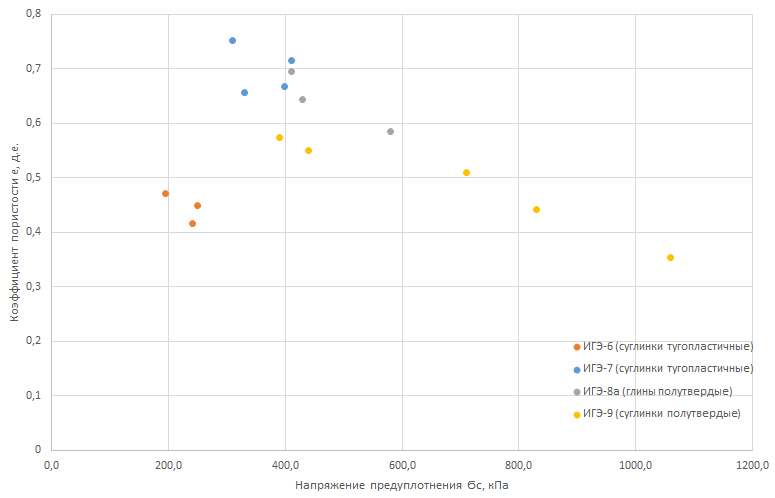
\includegraphics[scale=1]{1por.png}
  }
  \caption{График зависимости напряжения предуплотнения $\sigma_c$ от коэффициента пористости $e$ (метод Казагранде)}\label{fig:1por}
\end{figure}

\begin{figure}[h!]
  \centerfloat{
    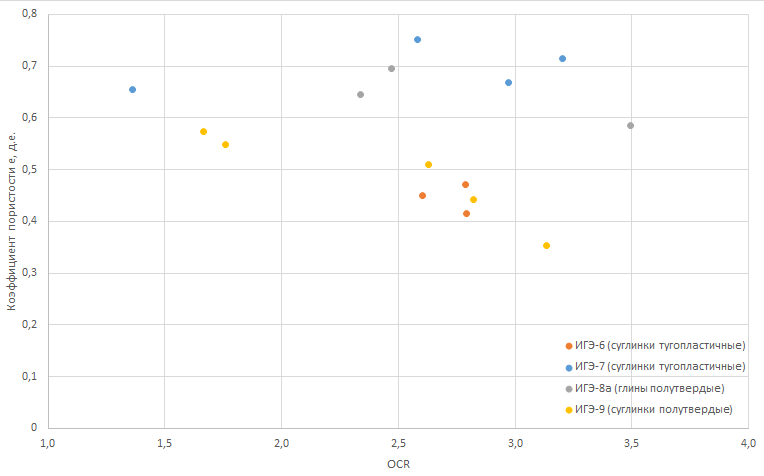
\includegraphics[scale=1]{3por.png}
  }
  \caption{График зависимости коэффициента переуплотнения $OCR$ от 
  коэффициента пористости $e$ (метод Казагранде)}\label{fig:3por}
\end{figure}

\begin{figure}[h!]
  \centerfloat{
    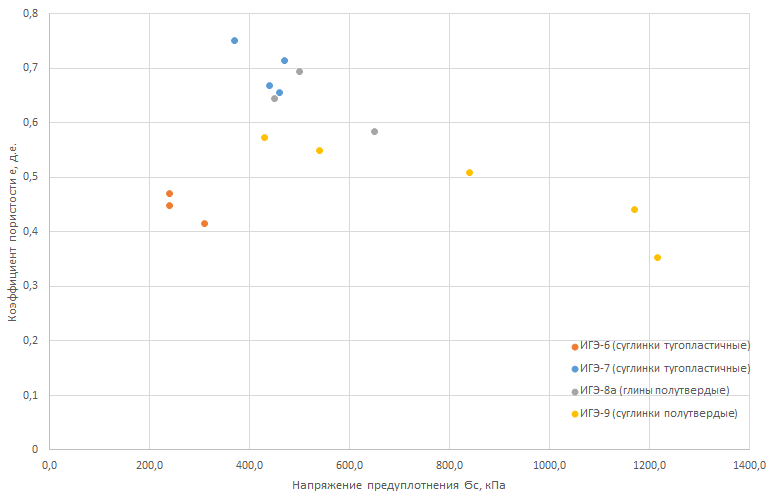
\includegraphics[scale=1]{11por.png}
  }
  \caption{График зависимости напряжения предуплотнения $\sigma_c$ от 
  коэффициента пористости $e$ (метод Беккера)}\label{fig:11por}
\end{figure}

\begin{figure}[h!]
  \centerfloat{
    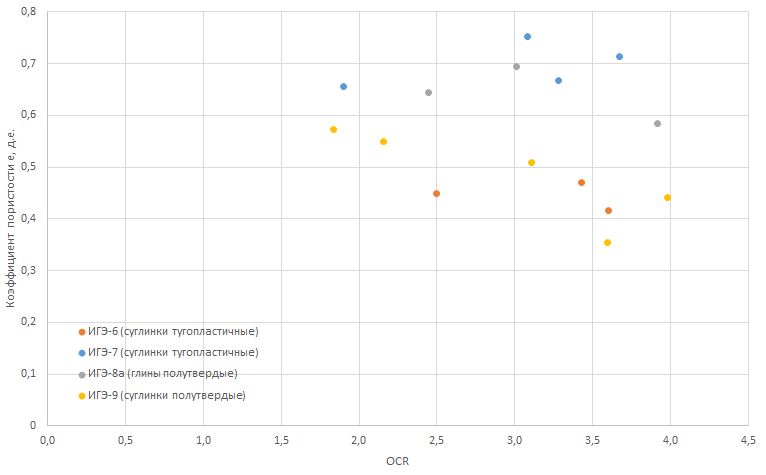
\includegraphics[scale=1]{33por.png}
  }
  \caption{График зависимости коэффициента переуплотнения $OCR$ от 
  коэффициента пористости $e$ (метод Беккера)}\label{fig:33por}
\end{figure}

%\section{Характеристика ледниковых отложений донского горизонта}
%
%Ледниковые отложения донского горизонта g~I~ds характеризуются следующим
%минеральным составом: хлорит =$\thicksim$2,9\%, смектит =$\thicksim$13,75\%, 
%иллит =$\thicksim$6,8\%, палыгорскит =$\thicksim$0,55\%, 
%каолинит =$\thicksim$2,75\%, кварц =$\thicksim$48,55\%,
%КПШ (микроклин, ортоклаз) =$\thicksim$8,85\%, 
%плагиоклазы (альбит, андезит) =$\thicksim$5,30\%, 
%кальцит =$\thicksim$4,15\%, доломит =$\thicksim$5,30\%,
%пирит =$\thicksim$ 0,35\%, амфиболы (роговая обманка) =$\thicksim$0,75\%.
%Минералов сидерит и рутил в грунтах донского горизонта 
%не обнаружено.
%
%Рассматриваемые отложения имеют 
%гранулометрический состав, по которому по 
%классификации В.В.Охотина грунт можно назвать 
%суглинком средним. 
%
%Осредненные физические свойства  грунтов 
%донской морены представлены в таблице \ref{tab:donfiz}.
%
%\begin{table}[]
%  \small
%  \centering
%  \caption{Физические свойства ледниковых отложений донского горизонта}\label{tab:donfiz}
%  \begin{tabular}{|c|l|}
%  \hline
%  \multicolumn{1}{|l|}{Характеристика} & Значение \\ \hline
%  $W$, \%                                & 17       \\ \hline
%  $W_L$, \%                               & 33       \\ \hline
%  $W_P$, \%                               & 15       \\ \hline
%  $I_p$, д.е.                             & 0,18     \\ \hline
%  $I_l$, д.е.                             & 0,12     \\ \hline
%  $\rho$, г/см3                             & 2,15     \\ \hline
%  $\rho_s$, г/см3                            & 2,71     \\ \hline
%  $e$, д.е.                              & 0,48     \\ \hline
%  $S_r$, д.е.                             & 0,94     \\ \hline
%  \end{tabular}
%  \end{table}
% 
% Осредненные характеристики 
% переуплотнения по методам и Казагранде, 
% и Беккера представлены в таблице \ref{tab:donmeh}.
%
% \begin{table}[]
%  \small
%  \centering
%  \caption{Параметры переуплотнения ледниковых отложений донского горизонта}\label{tab:donmeh}
%  \begin{tabular}{|c|l|l|}
%  \hline
%  \multicolumn{1}{|l|}{Характеристика} & Метод Казагранде & Метод Беккера \\ \hline
%  $\sigma_0$, кПа                              & \multicolumn{2}{c|}{277,2}       \\ \hline
%  $\sigma_c$, кПа                              & 686,0            & 839,0         \\ \hline
%  $POP$, кПа                             & 408,8            & 561,8         \\ \hline
%  $OCR$                                  & 2,4              & 2,9           \\ \hline
%  \end{tabular}
%  \end{table}